\documentclass[10pt,openany,letterpaper]{article}
\usepackage{graphicx}
\usepackage{tikz}
\usepackage{enumitem}
\usepackage{amssymb}
\usepackage{amsmath}
\usepackage{xcolor}
\usepackage{color, colortbl}
\newcommand*{\defeq}{\stackrel{\text{def}}{=}}
\title{Tugas Aljabar I}
\author{Teosofi Hidayah Agung\\
5002221132}
\date{}
\begin{document}
\maketitle
\pagenumbering{gobble}
\setlength{\belowdisplayskip}{-4.5mm}
\setlength{\abovedisplayskip}{1.5mm}
\allowdisplaybreaks
    \begin{enumerate}
    \item 
    \begin{enumerate}
        \item Tentukan semua elemen dari $D3$.\\
        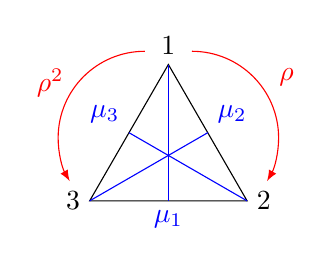
\begin{tikzpicture}
        \coordinate[label=above:1] (A) at (3,1.732050807568877);
        \coordinate[label=right:2] (B) at (4,0);
        \coordinate[label=left:3] (C) at (2,0);
        \coordinate[label=below:$\color{blue}\mu_1$] (M1) at (3,0);
        \coordinate[label=above right:$\color{blue}\mu_2$] (M2) at (3.5,0.866025);
        \coordinate[label=above left:$\color{blue}\mu_3$] (M3) at (2.5,0.866025);

        
        \draw (C)--(A)--(B)--cycle;
        \draw[blue] (A)--(M1);
        \draw[blue] (C)--(M2);
        \draw[blue] (B)--(M3);

        \draw[-latex,red] (3.3,1.9) arc
            [
            start angle=90,
            end angle=-30,
            x radius=1.1cm,
            y radius =1.1cm
            ] ;
        \coordinate[label=below:$\color{red}\rho$] (R1) at (4.5,1.8);
        \coordinate[label=below:$\color{red}\rho^2$] (R1) at (1.5,1.8);
        \draw[-latex,red] (2.7,1.9) arc
            [
            start angle=90,
            end angle=210,
            x radius=1.1cm,
            y radius =1.1cm
            ] ;
    \end{tikzpicture}
    \begin{flalign*}
        \rho_0&=\begin{pmatrix}1\end{pmatrix}&\\
        \rho&=\begin{pmatrix}1&2&3\end{pmatrix}&\\
        \rho^2&=\begin{pmatrix}1&3&2\end{pmatrix}&\\
        \mu_1&=\mu=\begin{pmatrix}2&3\end{pmatrix}&\\
        \mu_2&=\rho\mu=\begin{pmatrix}1&2\end{pmatrix}&\\
        \mu_3&=\rho^2\mu=\begin{pmatrix}1&3\end{pmatrix}&\\
        D_3&=\{\rho_0,\rho,\rho^2,\mu_1,\mu_2,\mu_3\}&\\
    \end{flalign*}\\
    \item Buatlah tabel dari $D3$.\\
    \newcolumntype{l}{>{\columncolor{lime}}c}
    \begin{center}
    \begin{tabular}{|l|| c c c c c c|} 
        \hline
        \rowcolor{cyan}
         \color{purple}$\circ$ & $\rho_0$ & $\rho$ & $\rho^2$ & $\mu_1$ & $\mu_2$ & $\mu_3$\\
         \hline\hline
         $\rho_0$ & $\rho_0$ & $\rho$ & $\rho^2$ & $\mu_1$ & $\mu_2$ & $\mu_3$\\
         $\rho$ & $\rho$ & $\rho^2$ & $\rho_0$ & $\mu_2$ & $\mu_3$ & $\mu_1$\\
         $\rho^2$ & $\rho^2$ & $\rho_0$ & $\rho$ & $\mu_3$ & $\mu_1$ & $\mu_2$\\
         $\mu_1$ & $\mu_1$ & $\mu_3$ & $\mu_2$ & $\rho_0$ & $\rho^2$ & $\rho$\\
         $\mu_2$ & $\mu_2$ & $\mu_1$ & $\mu_3$ & $\rho$ & $\rho_0$ & $\rho^2$\\
         $\mu_3$ & $\mu_3$ & $\mu_2$ & $\mu_1$ & $\rho^2$ & $\rho$ & $\rho_0$\\
         \hline
    \end{tabular}
    
    \vspace{0.9mm}
    Tabel komposisi
    \end{center}

    \item Dari tabel tentukan $(\rho\mu)^{-1}$ dan $(\rho^2\mu)^{-1}$.\\
    \begin{flalign*}
        (\rho\mu)^{-1}&=(\mu_2)^{-1}=\mu_2=\rho\mu&\\
        (\rho^2\mu)^{-1}&=(\mu_3)^{-1}=\mu_3=\rho^2\mu&\\
    \end{flalign*}
    \end{enumerate}

    \item $(D_5,\circ)$ grup dehidral.\\
    $f,g,h,i \in D_4$
    \begin{flalign*}
        f&=\rho\mu&\\
        g&=\rho^3&\\
        h&=\rho^2\mu&\\
        i&=\rho^3\mu
    \end{flalign*}
    \begin{enumerate}[label=(\roman*)]
        \item Tentukan $k$ dimana
        \begin{enumerate}[label=\textcircled{\alph*}]
            \item $f\circ g=\rho^k\mu$
            \begin{flalign*}
                (\rho\mu)\rho^3&=\rho^k\mu&\\
                (\mu\rho^3)\rho^3&=\rho^k\mu&\\
                \mu(\rho^3\rho^3)&=\rho^k\mu&\\
                \mu\rho^2&=\rho^k\mu&\\
                \rho^2\mu&=\rho^k\mu&\\
                \therefore k=2
            \end{flalign*}
            \item $g\circ f=\rho^k\mu$
            \begin{flalign*}
                \rho^3(\rho\mu)&=\rho^k\mu&\\
                \rho_0\mu&=\rho^k\mu&\\
                \therefore k=0
            \end{flalign*}
            \item $h\circ i=\rho^k\mu$
            \begin{flalign*}
                (\rho^2\mu)(\rho^3\mu)&=\rho^k\mu&\\
                \rho^2(\mu\rho^3)\mu&=\rho^k\mu&\\
                \rho^2(\rho\mu)\mu&=\rho^k\mu&\\
                (\rho^2\rho)(\mu\mu)&=\rho^k\mu&\\
                (\rho^3)(\mu\mu)\mu^{-1}&=\rho^k\mu\mu^{-1}&\\
                \rho^3\mu&=\rho^k&\\
                \therefore \textrm{tidak ada }k \textrm{ yang memenuhi}
            \end{flalign*}
            \item $i\circ h=\rho^k\mu$
            \begin{flalign*}
                (\rho^3\mu)(\rho^2\mu)&=\rho^k\mu&\\
                \rho^3(\mu\rho^2)\mu&=\rho^k\mu&\\
                \rho^3(\rho^2\mu)\mu&=\rho^k\mu&\\
                (\rho^3\rho^2)(\mu\mu)&=\rho^k\mu&\\
                (\rho)(\mu\mu)\mu^{-1}&=\rho^k\mu\mu^{-1}&\\
                \rho\mu&=\rho^k&\\
                \therefore \textrm{tidak ada }k \textrm{ yang memenuhi}
            \end{flalign*}
        \end{enumerate}
        \item Tentukan $h^{-1},g^{-1}$
        \begin{flalign*}
            h^{-1}&=(\rho^2\mu)^{-1}&\\
            &=(\mu)^{-1}(\rho^2)^{-1}&\\
            &=\mu\rho^2&\\
            &=\rho^2\mu&\\
            g^{-1}&=(\rho^3)^{-1}&\\
            &=\rho&\\
        \end{flalign*}
    \end{enumerate}
    \item $f,g\in S_7$ dimana
    \begin{align*}
        f&=\begin{pmatrix}1&3&4\end{pmatrix}\begin{pmatrix}2&5&7&6\end{pmatrix}\\
        g&=\begin{pmatrix}2&3&5\end{pmatrix}\begin{pmatrix}1&4&7\end{pmatrix}\\
    \end{align*}
    Nyatakan hasil berikut dalam komposisi sikel yang saling asing.
    \begin{enumerate}[label=\textcircled{\alph*}]
        \item $f\circ g$
        \begin{flalign*}
            &\begin{pmatrix}1&3&4\end{pmatrix}\begin{pmatrix}2&5&7&6\end{pmatrix}\circ\begin{pmatrix}2&3&5\end{pmatrix}\begin{pmatrix}1&4&7\end{pmatrix}&\\
            &=\begin{pmatrix}1\end{pmatrix}\begin{pmatrix}2&4&6\end{pmatrix}\begin{pmatrix}3&7\end{pmatrix}\begin{pmatrix}5\end{pmatrix}&\\
            &=\begin{pmatrix}2&4&6\end{pmatrix}\begin{pmatrix}3&7\end{pmatrix}&\\
        \end{flalign*}
        \item $g\circ f$
        \begin{flalign*}
            &\begin{pmatrix}2&3&5\end{pmatrix}\begin{pmatrix}1&4&7\end{pmatrix}\circ\begin{pmatrix}1&3&4\end{pmatrix}\begin{pmatrix}2&5&7&6\end{pmatrix}&\\
            &=\begin{pmatrix}1&5\end{pmatrix}\begin{pmatrix}2\end{pmatrix}\begin{pmatrix}3&7&6\end{pmatrix}\begin{pmatrix}4\end{pmatrix}&\\
            &=\begin{pmatrix}1&5\end{pmatrix}\begin{pmatrix}3&7&6\end{pmatrix}&\\
        \end{flalign*}
        \item Apakah $f\circ g=g\circ f$?\\
        Tidak, karena fakta bahwa sikel-sikel dalam $f$ dan $g$ tidak saling asing, sehingga dapat dilihat dari \textcircled{a} dan \textcircled{b} bahwa $f\circ g\neq g\circ f$.
    \end{enumerate}
    \end{enumerate}
    
\end{document}